\documentclass{article}


% if you need to pass options to natbib, use, e.g.:
%     \PassOptionsToPackage{numbers, compress}{natbib}
% before loading neurips_2022


% ready for submission
%\usepackage{setup/neurips_2022}


% to compile a preprint version, e.g., for submission to arXiv, add add the
% [preprint] option:
\usepackage[preprint]{setup/neurips_2022}


% to compile a camera-ready version, add the [final] option, e.g.:
%     \usepackage[final]{setup/neurips_2022}


% to avoid loading the natbib package, add option nonatbib:
%    \usepackage[nonatbib]{setup/neurips_2022}


\usepackage[utf8]{inputenc} % allow utf-8 input
\usepackage[T1]{fontenc}    % use 8-bit T1 fonts
\usepackage{hyperref}       % hyperlinks
\usepackage{url}            % simple URL typesetting
\usepackage{booktabs}       % professional-quality tables
\usepackage{amsfonts}       % blackboard math symbols
\usepackage{nicefrac}       % compact symbols for 1/2, etc.
\usepackage{microtype}      % microtypography
\usepackage{xcolor}         % colors


% The \author macro works with any number of authors. There are two commands
% used to separate the names and addresses of multiple authors: \And and \AND.
%
% Using \And between authors leaves it to LaTeX to determine where to break the
% lines. Using \AND forces a line break at that point. So, if LaTeX puts 3 of 4
% authors names on the first line, and the last on the second line, try using
% \AND instead of \And before the third author name.


\author{
  Shao-Ting Chiu\thanks{UIN: 433002162} \\
  Department of Electrical and Computer Engineering\\
  Texas A\&M University\\
  College Station, TX 77843 \\
  \texttt{stchiu@tamu.edu} \\
  \AND
  Chan-Min Hsu\thanks{UIN: 532008407} \\
  Department of Electrical and Computer Engineering\\
  Texas A\&M University\\
  College Station, TX 77843 \\
  \texttt{chanminhsu@tamu.edu} \\
}



\title{Predicting Stock Market with Bayesian Neural Network}


\begin{document}

\maketitle


\begin{abstract}
The randomness of stock market challenge investments to be reliable. Many of approaches has been introduced to find the hidden pattern behind the transitions. However, error estimation with non-parametric method is in the early stage. In this project, we used Bayesian neural network to predict discrete  time-series data with moving window of kernel. The Monte Carlo Markov Chain method is applied to measure the posterior distribution. The purpose is to provide a model-free approach with uncertainty quantification that is essential to the investment strategy. 
\end{abstract}

\section{Introduction}

\section{Methods}



\section{Dataset}

\paragraph{The dataset} contains the closing price per day for 4 stocks in 4 countries (Table \ref{tab:my_label}). These discrete time-series data is processed by normalization ($x_{i}' = \frac{x_{i} - x_{\min}}{x_{\max} - x_{\min}}$). The dataset is labeled by two timeframes: before and during COVID-19. Suppose the closing stock price is $[x_1, \dots, x_N]$ where $N$ is the length of the time series, the purpose is to predict the time series after the first few days of COVID-19 spreading.



The original data set is $x_t = \{x_{1}, ..., x_{Total}\}$, the training input is a matrix with dimension $m \times s$ (where m is the capture window, and $s$ is the number of samples). The sample is produced by shifting the original time series with lag of $2$.  These discrete time-series data is processed by normalization ($x_{i}' = \frac{x_{i} - x_{\min}}{x_{\max} - x_{\min}}$). 

\begin{equation}
\bar{x}_t = 
\underbrace{\begin{bmatrix}
    x_{1+(t-1)T} & \cdots & x_{m+(t-1)T}\\
    x_{3+(t-1)T} & \cdots & x_{2m+3+(t-1)T}\\
    \vdots & \vdots & \vdots 
\end{bmatrix}}_{\text{m(Capture windows)}}
\end{equation}

\begin{equation}
y_t = 
\underbrace{\begin{bmatrix}
    x_{m+(t-1)T + 1} & \cdots & x_{m+(t-1)T+ n}\\
    x_{2m+3+(t-1)T + 1} & \cdots & x_{2m+3+(t-1)T+ n}\\
    \vdots & \vdots & \vdots
\end{bmatrix}}_{\text{n (Prediction Horizons)}}
\end{equation}


\begin{figure}
     \centering
     \begin{subfigure}[b]{0.5\textwidth}
         \centering
         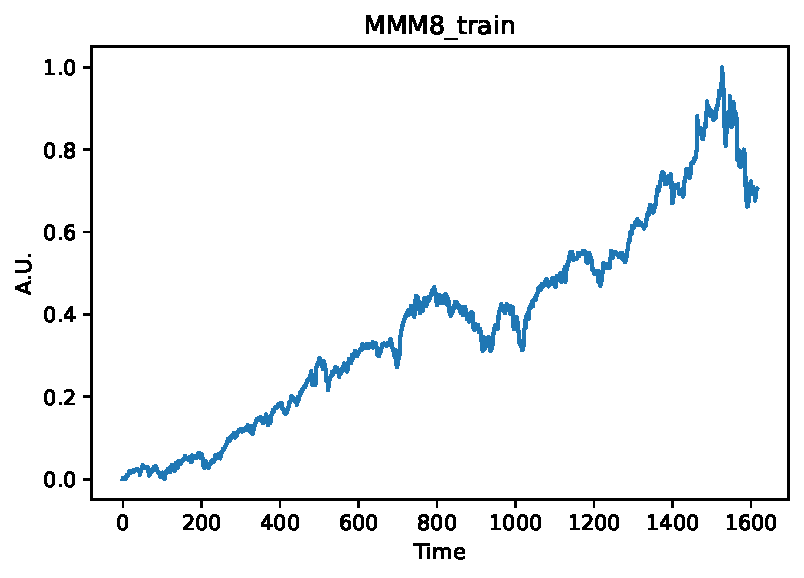
\includegraphics[width=\textwidth]{../img/MMM8_train.pdf}
         \caption{Train set (before COVID-19)}
     \end{subfigure}%
     \begin{subfigure}[b]{0.5\textwidth}
         \centering
         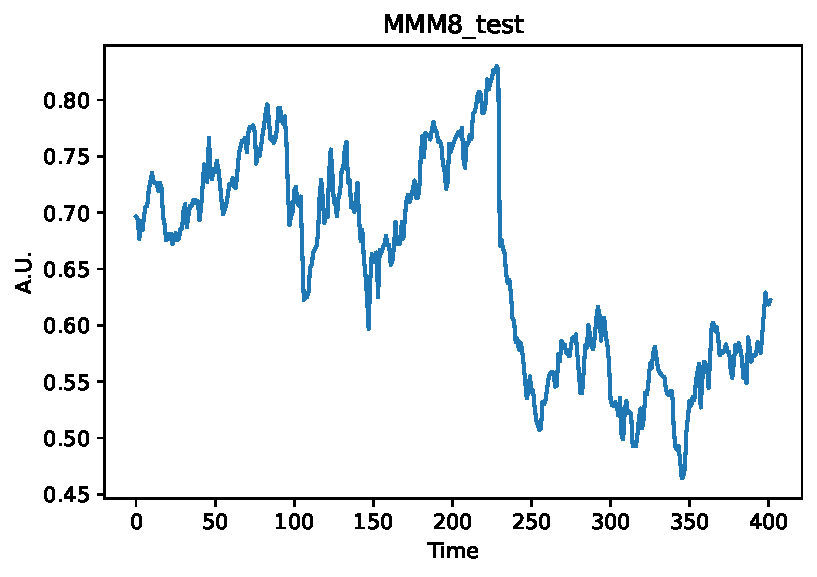
\includegraphics[width=\textwidth]{../img/MMM8_test.pdf}
         \caption{Test set (before COVID-19)}
     \end{subfigure}
     \hfill
     \begin{subfigure}[b]{0.5\textwidth}
         \centering
         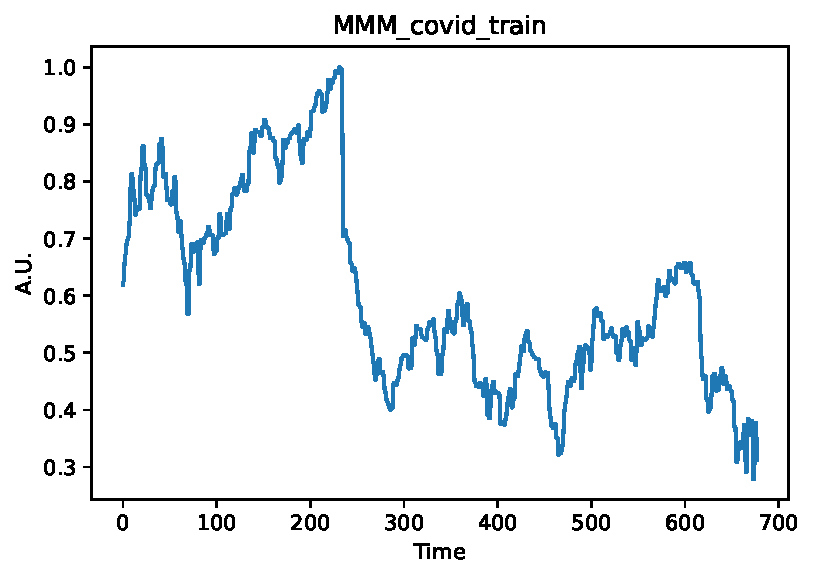
\includegraphics[width=\textwidth]{../img/MMM_covid_train.pdf}
         \caption{Train set during COVID-19}
     \end{subfigure}%
     \begin{subfigure}[b]{0.5\textwidth}
         \centering
         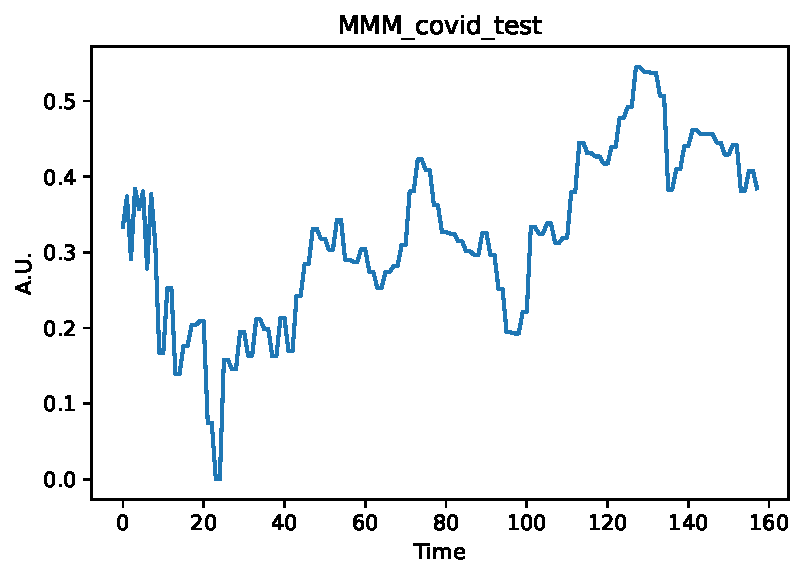
\includegraphics[width=\textwidth]{../img/MMM_covid_test.pdf}
         \caption{Test set during COVID-19}
     \end{subfigure}
    \caption{Stock markets of a company before and during COVID-19 \cite{chandra2021bayesian}.}
    \label{fig:data-series}
\end{figure}



\bibliography{ref}

\end{document}